\chapter{Implementation}

The implementation of the design of this application followed an iterative methodology, with builds moving slowly towards the design that has been described in the previous chapter. This chapter will break the application's development into distinct iterations, with the initial iteration being what was considered the Minimum Viable Product - that being that the software had fulfilled the essential requirements and its core functionality had been implemented. Each iteration will include a subsection, that defines what was included in the design at that point. The final iteration will have included all facets of the design.

\section{Iteration I: Minimum Viable Product}
\subsection{Design}
The Minimum Viable Product for the purposes of this project was defined to be the successful completion of user stories 1 and 3 (see Appendix A). In this iteration, a user interface which includes a map, that has markers on it, is created, and the markers are able to be clicked on to show their name and their description. Two forms were also created in this iteration; one form to add a point of interest, and another to edit a given point of interest. Notably, no authentication or geocoding was present in this iteration, with any user being given the ability to add or edit a point of interest.

At this stage, data and backend layers for user authentication had not been implemented. The application consisted of two views - one view containing the homepage, and the other containing a form for adding and editing a point of interest. However, all elements of the technology stack were used to implement this iteration.
\newpage


\subsection{Google Maps for JavaScript API}

The main part of this iteration was the implementation of the Google Maps for JavaScript API, and research into how this needs to be implemented. Google provides a large set of documentation detailing possible uses for the API, as well as a tutorial on how to use it.

One important part of the implementation of the API involves the use of an API key, for authentication. This API key is linked to an account holder, with any deductions over the monthly limit being automatically invoiced to the account holder on a monthly basis by Google. The issues caused by using a Google Cloud API key are, first and foremost, the lack of the ability to transfer the API key to a customer's account, as well as the complexity of the Google Cloud interface. There are many ways in which an account holder, who may have not used cloud-based deployment platforms before, could accidentally make large purchases. Powerful 'one-click' virtual machines can be deployed in a matter of seconds, but can be very costly if not shutdown.

To mitigate this issue, restrictions were placed on the API key, that only permitted its use for requests made through its JavaScript API, and there was no authorisation for transactions over the free monthly allowance. As discussed in section~\ref{sec:googlemaps}, there is little likelihood for requests made to the API to exceed this allowance, if used solely on this application. This also reduces the likelihood of attackers, who may have extracted the API key from the source code of the homepage, being able to carry out any meaningful damage, as the API key can be easily swapped with another account, if needs be.

The core of the API implementation consists of a callback function, \texttt{async function initMap()}, that is called asynchronously as the homepage loads. The code for this is stored in a separate file, \texttt{googlemaps.js}. The function utilises the API to instantiate a map, which is then populated with points of interest through an iterative for loop. The points of interest are found through use of JavaScript's Fetch API, an interface that allows for fetching of resources. An API call is made to a method which returns all points of interest that are currently in the database.

A problem faced when implementing this part of the application was the element of difficult whilst debugging parts of the JavaScript. Google Chrome and Mozilla Firefox's debugging tools were used, however it was often difficult to pinpoint the exact issue, due to the inability to debug the function calls from Google's API. Ensuring that the click listener was correctly appended to each marker also required some prior readings into utilising JavaScript for this. Ensuring that the code was clean was also a challenge during the refactoring, with attempts made to stop code leakage and ensure the procedural programming that was being used throughout the JavaScript element of this project remained.

\subsection{Backend}

The backend of the application retained the simple database layer at this iteration - an un-normalised table of points of interest. In order to ensure it interfaced correctly with the database, Java Persistence API annotations had to be used. \texttt{@Entity} is an example of annotation used on \texttt{PointOfInterest}, that declares the object as an entity that has an identical relation in the database. Spring's configuration properties also had to be edited, to ensure the database that had been manually created is not dropped and replaced with Hibernate's impression of the database. However, constraints were also added directly to the object, via JPA annotations. One example is the \texttt{double latitude} member of the class. Two constraints were added to it, \texttt{@Min(value = -90, message = "Error: Latitude cannot be lower than -90")}, and \texttt{@Max(value = 90, message = "Error: Latitude cannot be greater than 90")}. These provide minimum and maximum constraints, and can pass a message if an exception is thrown, that can be shown at the view layer.

The class had to be implemented in such a way as it could be easily consumed by the data layer, without having to manually call the object's setters and passing each attribute of the form as a single attribute. The JPA allows for automatic setting of class members through either a constructor or setters. In this iteration, a constructor was used. However, setters and getters had also been created to improve the functionality of the code and assist in getting private members in other parts of the application; a unit test, for example.

In this iteration, the controller layer of the application interfaced directly with the database, as opposed to using the service layer to encapsulate the logic of the application. The application was relatively simple at the time, so it was decided that it wouldn't be necessary for an MVP to include that layer, as it would essentially be repeating repository methods without any further work carried out to the object. Spring's \texttt{@RestController} annotation, that provides controller functionality without methods being required to return a view, allowed for a RESTful API to be created without much more configuration than would be required if a standard controller was made. At that point, a \texttt{PageController}, carrying the \texttt{@Controller} annotation, had also been created to permit navigation between simple parts of the app, that did not require a model to be attached to it - the homepage, for example. In this iteration, the RESTful API created a method to list all points of interest, through utilising the \texttt{findAll()} method in JPA repositories, and add a point of interest to the database.

Difficulties were faced with creating a distinction between adding a point of interest and updating a point of interest. The \texttt{save()} method in JPA repositories will perform an SQL UPDATE, as opposed to an SQL INSERT, operation, if the primary key of the given object matches that of one object in the database. Relying on this, however, seemed to result in a conflict exception. A workaround was implemented - a second, distinct, update method and API mapping was created. This took two arguments, the Point of Interest with its updated members, and the ID of the point of interest. The ID would then have to be set within the method to allow for the SQL UPDATE operation to be triggered - with the conclusion being that the ID of any point of interest is lost within its transmission from the view layer to the controller layer.

\subsection{Frontend}

A number of challenges were posed when scripting the frontend of the application, including following Materialize's standards for layout development, and utilising Thymeleaf correctly and efficiently.

Thymeleaf's implementation in Spring focuses on a ``resources" folder, with two subfolders, ``static" and ``template". The first folder, as the name suggests, contains static resources - resources that Thymeleaf and Spring would not change at compile time. This included \texttt{materialize.css}, the CSS file that provides implementation of each Materialize UI components, with the JavaScript containing Materialize's JavaScript helper functions, the Google Maps function discussed above, as well as a third-party algorithm, ``lazysizes"\cite{lazysizes}. This implements the lazy-loading algorithm on images that are assigned this class; the algorithm ensuring that the resource attached to it is only loaded when required. In this instance, the algorithm was applied to images in the marker popup, to ensure they were not loaded before required, which would impact initial page load times.

The second folder contains the HTML for pages that are to be rendered onto the browser. Thymeleaf expects HTML to be typed declaratively, as opposed to approaches frameworks such as React take. A feature of Thymeleaf, that was researched and used during this iteration, is its fragments feature. This feature allows you to place reused code into its own file, and called at the position that it would be written in a static HTML website. For example, calls to files such as Material Icons were placed in \texttt{fragments/header.html}, and, in the \texttt{<head>} tags of all templates, it was called with the line \texttt{<fragment th:replace
="fragments/header :: header"></fragment>}. When this was rendered in the browser, the source would show what was in the fragment. This allowed for less reused code, and easier navigability within the resources files.

Correct placement of the map seemed to pose an issue when creating the homepage. The container for the Maps JavaScript appeared to overflow the page's default view height, requiring a user to scroll down to be able to view it. This was not a reasonable expectation for the user, particularly as it was intended to be used in a web browser set to full-screen. A workaround for this was implemented, by creating a custom CSS file. This CSS file overrode Materialize's grid system by having the height be declared manually, with the line being \texttt{height: calc(99vh - 56px);}. The height of the menu bar, at the top of the screen, measured at fifty-six pixels, according to the CSS file. With a view height of 100 still appearing to overflow the page, decrementing this by one appeared to resolve the issue, and showed an aesthetically pleasing home screen.

The `admin panel', at this stage, had two forms, one to add a point of interest, and one to edit a point of interest. Research had to take place in how to correctly manage a POST request within an HTML form when using Thymeleaf. The Thymeleaf XML namespace allowed you to call the backend from the view. Therefore, in the 'add' form, Thymeleaf calls the HTTP POST method in the controller, and instantiates an empty POI with \texttt{th:object="\$\{pointOfInterest\}"}. Each field within the HTML form also included a Thymeleaf attribute, \texttt{th:field}, that included the member of the POI object that the field relates to. This was similar in the edit form, with a duplicate form being used that is instead populated with members from the point of interest provided in the model of the view.

\begin{figure}[H]
	
\includegraphics[scale=1.0]{diagrams/listPOI}
	\caption{An example of a point of interest list in the view layer.}
\end{figure}	


A list of points of interests also had to be made, which included edit and delete buttons for every point of interest. This was created through performing iteration within Thymeleaf, with a method call to the GET request that returns all points of interest in the database. This is called within a list object in the view as \texttt{th:each="poi : \${pointsOfInterest}"}, and is populated at runtime, with the rendered view containing every point of interest. This allows for simplicity to be achieved in the view, and negates the need for JavaScript, as an example, to be used, reducing the amount of code within one view.
% 1995 words
% Total: 8562 words
% Remaining: 3438 words

\section{Iteration II: Admin authentication}
\subsection{Design}

The second iteration of the application focused on implementing authentication for the admin panel. The previous iteration did not have any authentication - this would cause issues at production due to the web app being used in a public location. Therefore, this iteration fulfils story 2, and explored different authentication methods for only part of an application, rather than the entire application.

This stage implemented most of the backend and data layers described in chapter 2, however filtering and geocoding had still not been implemented at this stage. However, further parts of the frontend were implemented, with options to add and delete users from the admin panel.

\subsection{Spring Security}

This was the first iteration to take advantage of Spring Security, a security add-on that interfaces with the Spring Framework, as discussed in chapter 2. The main challenge posed when utilising Spring Security was ensuring that it linked correctly with the database layer. By default, Spring Security worked off of the basis of an in-built User object in the \texttt{org.springframework.security.core.userdetails} package. While this implementation included a username and password; the required fields if keeping to the design standard for this iteration, there was little way to customise its behaviour as well as use a custom \texttt{UserDetails} implementation. This facilitated the creation of a custom User and Role class, along with \texttt{UserDetailsServiceImpl}, a class that implements Spring \texttt{UserDetailsService} interface.

Another challenge when working with Spring Security was implementing an acceptable storage method for sensitive personal data. After reviewing the customer's requirements, it was decided that only a username and an encrypted password should be stored. This fit with the customer's requirements, with the main aim of authentication being that the add/edit forms are inaccessible to the general public. It also stops any legal concerns that could arise from the storage of personal data such as full names, e-mail addresses and telephone numbers, a data set that could arguably be legislated by data protection laws in the UK\cite{dpa2018}.

It would have not been acceptable to store passwords as plain text. Spring Security accepts plain-text passwords by default, and an algorithm has to be implemented to encrypt passwords. As discussed in section~\ref{springpassword}, classes for a one-way hashing algorithm needed to be explored, and one was picked that had been proven to be reasonably difficult to crack.

Unpredictable behaviour occurred when a user was registered with the same name as another user in the database. As discussed in chapter 2, there was more efficiency using a numerical sequence as a primary key, then there would have been if a string was used, as may had been the case in many common implementations of a user relation. Without any constraints or exception handling, two users were able to be created with the same username. Exceptions were thrown at the Spring layer should you attempt to login with a duplicate username. To work around this issue, a unique constraint was added to the database for the username column. This was matched in the controller classes of Spring Security to an exception handler. The exception handler catches \texttt{DataIntegrityViolation.class}, an exception that is thrown when a conflict is detected in the database. The exception is handled by display an Error 400 page, with details of what occurred available to the user, and the opportunity to try again with a different username is given.

Initial setup of Spring Security appeared to have it default to requesting a login for access to any part of the web app, including the map. This would've defeated its purpose, given a member of the public could then access the admin panel regardless. This was modified through the use of a class that extends Spring's \texttt{WebSecurityConfigurerAdapter}, in its \texttt{configure(HttpSecurity http)} method. The source code of this method is available in Appendix C, section~\ref{securitymethod}. The use of matchers enabled all users to access the index page, that contains the map, and permitted that map to access any required resources. The line \texttt{.antMatchers("/admin/**").hasRole("ADMIN")} ensured that only registered users; automatically given the role of admin, are able to access the admin panel. The security configuration also enabled CSRF tokens. These tokens reduced the threat of cross-site request forgery, by appending tokens to authorised HTTP requests and disallowing requests that failed to include a valid token.
\newpage
\subsection{Backend}

Modifications had to be made to the backend to accommodate for Spring Security, as well as management of routing between various parts of the admin panel.

Similar to points of interest, the admin panel now included a form to register a new user, as well as a form to list all users and delete ones as appropriate. This required the creation of controllers for both the admin side of the application (that facilitated requests to the authenticated \texttt{/admin} URI), and an API to control requests made to the user relation in the database. Similar definitions to the point of interest API were created, including returning a list of all users in the database, and returning a form to add details to an empty user object. The user service encoded the password, received in plain text by the POST request, before storing it in the database.

Issues with infinite recursion occurred when a request was made to list all users. The User object contains a many-to-many relationship with a Role, allowing one user to be assigned more than one role. Whilst this functionality is not being used in this application, it was decided to maintain this relationship, in case further iterations past the first production build introduced different roles. The stack trace of the stack overflow error thrown when calling this request revealed that the error was due to how the Jackson JSON parsing API, included within Spring, was processing many-to-many relationships, adding the same role infinitely to the end of the JSON string of each user. This was resolved by appending the \texttt{@JsonIgnore} annotation on all members in the user field, apart from ID and username. The password was encrypted, though there was a marginal risk that the encrypted password could be used to access admin services through other means than an HTTP request. However, neither that or user roles had to be exposed outside of the authenticated areas that had been dictated by Spring security configuration.

\subsection{Frontend}

New pages had to be created, again to accommodate Spring Security. A similar strategy to points of interest was taken to the creation of these pages, including a page to register a user, and a page to list all users. Similar Thymeleaf methods for iteration and field injection were also utilised, with the registration form consuming the HTTP POST request to register a new user.

As explained in the discussion on Spring Security, exceptions had to be handled for duplicate usernames, as well as any other conflict exceptions. An error page was made to handle this, utilising Thymeleaf field injection methods to provide the user with an exception name and message. This can be used by the user to see if they had made any obvious mistakes when entering information (a duplicate username, for example), or could be passed to a support technician for debugging in any future releases.

The layout of these forms re-used concepts from the points of interest pages, with an emphasis on minimalism and ease-of-use. It was, however, decided not to include options for editing users - this was considered relatively futile due to the lack of information required to register a user, and there are seldom cases were only a user's username has to be changed. Some password managers, such as Google Password Manager, appeared to automatically fill the registration field with a saved username and password. It was difficult to decide on a way to stop this from happening, however, it is clear that the registration form registers a new user rather than logs a user in.

\section{Iteration III: Geocoding}
\subsection{Design}

The third iteration introduces geocoding to the software. Geocoding allows for an address, or part of an address, to be converted into a coordinate pair. Evaluation of different geocoding APIs is discussed in section~\ref{geocoding}, with an open-source API, Postcodes.io, used to geocode UK postcodes.

The customer for this web app is based in the UK, and they had mentioned that points of interest are likely to be local. Therefore, it was decided that a geocoding API that focuses solely on postcodes would be sufficient enough for the purposes of this application. While issues may arise with a postcode covering more than one location, a row of houses on a street, for example, it was deemed unlikely that points of interest would be in such places, particularly considering that the nature reserve in located in a rural area of Wales, where large, 'catch-all', postcodes are less likely than in urban areas.

This iteration introduces the postcode column to the point of interest relation, with constraints as discussed in chapter 2 being implemented. It also introduces classes to handle interfacing with the Postcodes.io API.

\subsection{Postcodes.io API}

The Postcodes.io API is an open-source interface with data from the Royal Mail and the Office of National Statistics, that provides various tools to work with the British postcode system. In this application, two of the tools were used, postcode-to-coordinate conversion, and the postcode validation tool.

Postcode-to-coordinate conversion allowed for a postcode to be queried in the API. The API returns a JSON string, containing characteristics specific to the postcode. An example of a postcode query is given below.

\begin{figure}[H]
	\begin{verbatim}
	{
    "status": 200,
    "result": [
        {
            "postcode": "SY23 3DB",
            "quality": 1,
            "eastings": 259560,
            "northings": 281846,
            "country": "Wales",
            "nhs_ha": "Hywel Dda University Health Board",
            "longitude": -4.066423,
            "latitude": 52.416527,
            "european_electoral_region": "Wales",
            "primary_care_trust": "Hywel Dda University Health Board",
            "region": null,
            "lsoa": "Ceredigion 002A",
            "msoa": "Ceredigion 002",
            "incode": "3DB",
            "outcode": "SY23",
            "parliamentary_constituency": "Ceredigion",
            "admin_district": "Ceredigion",
            "parish": "Aberystwyth",
            "admin_county": null,
            "admin_ward": "Aberystwyth Bronglais",
            "ced": null,
            "ccg": "Hywel Dda University Health Board",
            "nuts": "South West Wales",
            "codes": {
                "admin_district": "W06000008",
                "admin_county": "W99999999",
                "admin_ward": "W05000362",
                "parish": "W04000359",
                "parliamentary_constituency": "W07000064",
                "ccg": "W11000025",
                "ccg_id": "7A2",
                "ced": "W99999999",
                "nuts": "UKL14"
            }
        }
    ]
}
	\end{verbatim}
	\caption{An example of a result when querying the postcode SY23 3DB}
\end{figure}
	
As evidenced by the query, a large amount of information is returned, much of it not relevant for the purposes of this application. However, key-value pairs of longitude and latitude are of course of use in geocoding. Future iterations could perhaps benefit from other characteristics that can be derived from the postcode; an example perhaps being the "parish" key - this would contain the location that the postcode is in, and could be added to the information window.

Postcode validation is used to check that information can be derived from the string passed to the request, and returns a boolean confirming if it is valid or not. As discussed in chapter 2, this is used in place of a complex regular expression to ensure that edge cases; postcodes that are not valid however match the regular expression, are accounted for, and there is not a possibility of null pointers. Postcode validation also accounts for terminated postcodes, that at one point were valid however were changed, and may still be matched by a regular expression.

Consumption of the Postcodes.io API takes place in static methods within the \texttt{Postcode\\Service.java} class. An open-source Java library which contains methods that interface with this API is available, however, the requests made in this application are simple, therefore it was decided to use built-in Java and Spring libraries to avoid unnecessary addition of third-party libraries, that have potential to be unreliable or no longer be being updated by its authors. This class contains two static methods; one that checks if a postcode is valid and one that returns the coordinates of a given postcode, with two helper methods that encode a postcode as a UTF-8 string and returns the result of an HTTP request to the API. The \texttt{javax.net} library, which provides classes for networking, was used to return results from querying the API. The Jackson JSON processor; included by default with Spring, is used to handle the query and return the correct key-value pair. Another class used within this package is \texttt{Point2D.Double}, which allows for an X/Y coordinate pair to be passed in the same object.

\subsection{Backend}

Changes to the model and controller layers of the backend had to be made to facilitate postcode validation and entry. A nullable String object to hold postcodes was introduced as a member of the PointOfInterest class, with the latitude and longitude members of the class still being editable, should a user wish to enter a more precise location for a point of interest.

An issue arose around the inclusion of fields for both a postcode and coordinates. Without any changes being made, a user could potentially add both a postcode \textit{and} coordinates. The user-entered coordinates would override that of the postcode, rendering entry of the postcode futile. Therefore, the save method in \texttt{PointOfInterestService} was edited such that it would perform error-checking before geocoding the postcode and adding it to the database.

The error-checking strategy focused on both the latitude and longitude fields, and the postcode field. Should the latitude and longitude both be zero, a decision discussed in Chapter 2, the application would check if a postcode was entered, and then call the static service method to geocode the postcode, setting the coordinates through a helper method in the PointOfInterest class that assigns the relevant members of the returned Point2D.Double object to the latitude and the longitude. If no location was entered, or only one half of a coordinate pair was entered, this would violate the ``not null island" constraints, and a data integrity violation would be thrown. Conversely, a \texttt{PostcodeException}, a new subclass of \texttt{RuntimeException}, would be thrown, with the message that both a postcode and a set of coordinates were entered. \texttt{PostcodeException} is also thrown should an invalid postcode be entered.

\subsection{Frontend}

Changes to the forms for adding a point of interest, as well as exception handling templates, had to be designed in order to facilitate postcode entry. This took the shape of a ``location" section of the form, where it was specified that either a postcode or a pair of coordinates had to be entered, otherwise the aforementioned errors would occur.

Error handling took the same approach as previous iterations, with seldom changes required due to Thymeleaf's ability to inject the type of exception and the message that the exception carries into the template. 

% Words: 4272
% Total: 11051

\section{Iteration IV: Map additions and final build}

The final iteration, and the submitted build, of the application, generally fulfilled the tasks marked as ``Could have" - tasks that were not particularly necessary to include in the application in order for it to work well, however are useful additions, either for aesthetic reasons or conveniences.

Much of the work that took place in this iteration was on the Google Maps script. Third-party JavaScript libraries were utilised to implement marker clustering, that allowed for better visibility of markers. Filtering was also implemented, with changes to all parts of the stack to facilitate this.

A number of non-essential requirements were not able to be implemented in this final iteration. This will be briefly discussed in this section, and expanded upon in Chapter 5.

\subsection{Design}

This iteration completed the final build and implemented the design as described in Chapter 2. Differences to the previous iteration included the addition of a category column and member in the database and model layers respectively. Controller and service methods had to be updated to accommodate for this.

\subsection{Google Maps}

\texttt{googlemaps.js}, the implementation of the Google Maps API for this application, was edited to include the MarkerClustererPlus library. This is parts of Google's Maps Utility Library, and is accessed via a Content Delivery Network. Theoretically, it was possible to implement this library locally, however Google's recommended method of installation was via npm, a JavaScript package manager. As the JavaScript file was using a vanilla implementation of JavaScript, rather than taking a modular approach, common with ECMAScript 6 applications, it was difficult to download and include locally without major edits having to be made.

Marker clustering was relatively simple to implement. A group of marker images for various zoom levels was downloaded from Google's tutorial on the library, and the marker clusterer was instantiated at the beginning of the script. Markers were added to the cluster within the for-each loop that added information to each point of interest's information window.

The strategy for filtering markers involved creating a new function, and changing the marker and cluster arrays to global variables. When the user clicked on a filter, a function with the given category was called, and an iterative loop would be instigated. The loop would create a new array of markers, through checking each marker's category property within the array and setting the marker's visibility dependent on it matching the category given. User-level testing of these methods was successful, with options also added to clear any filtering and show all markers again. A function for a 'reset' button was also created. When the reset button was clicked, the map would pan back to the original location; centring on the Dyfi Wildlife Centre. Again, user testing proved that this works.

\subsection{Backend}

Changes had to be made to the backend to accommodate for a category to be added to each marker. Initially, this was to take the form of three booleans, \texttt{isWildlife}, \texttt{isBusiness}, and \texttt{isTransport}. Difficulties with this approach appeared centred on difficulties with Thymeleaf passing booleans from the view layer to the model; appearing to either return a string containing the value or not being able to discern the type of the field. An incompatibility between Thymeleaf and Materialize was also discovered - this is expanded upon further within the frontend subsection.

The workaround solution was to have the category hold a string, with a maximum length of the longest category. This was not a perfect solution, as it could have potentially allowed for any string to be entered if the HTTP request was edited in any way other than through the form. However, this was deemed a low risk - any object with a category that is not wildlife, business, or transport would appear if the filtering was set to all. It was already possible for a point of interest to have no category; this was a deliberate design to account for any point of interest that didn't fit with any of the defined categories. The time that would have been required to research an alternative solution outweighed the potential benefits of a more robust solution for filtering and categorisation.

\subsection{Frontend}
\begin{figure}[H]
	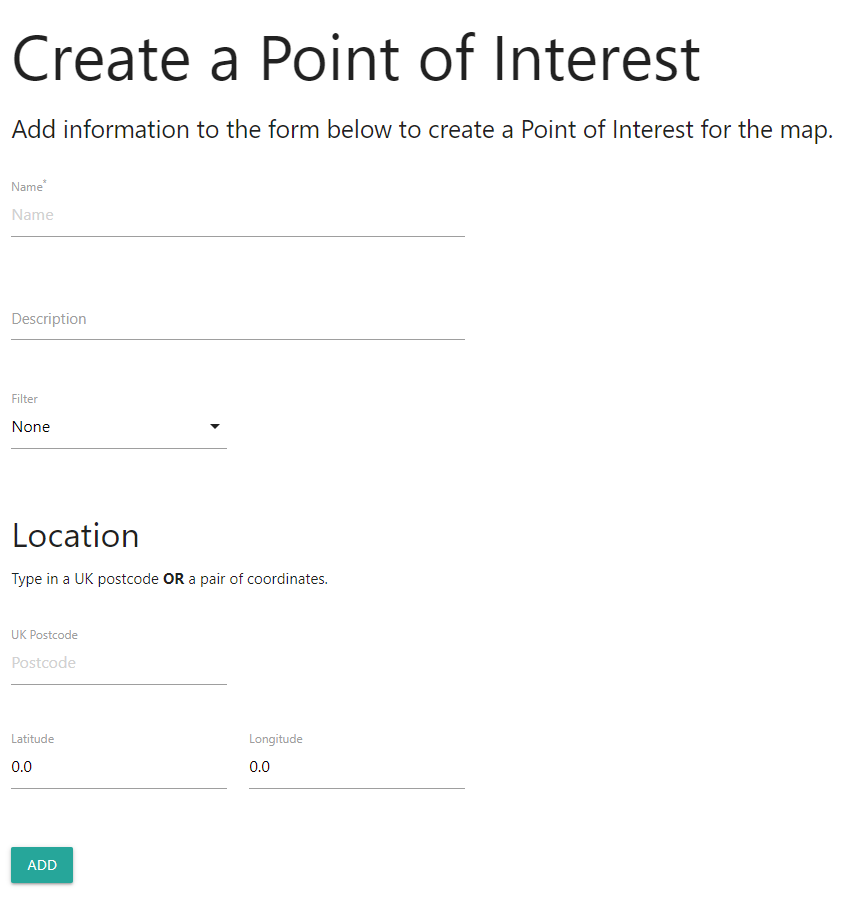
\includegraphics[scale=1.0]{diagrams/submittedForm}
	\caption{The 'Add a POI' form that is present in the final build of the application.}
\end{figure}	

Initially, errors were thrown when filtering was introduced to the frontend. The initial solution to modification of the add and edit point of interest forms was to include three checkboxes, one for each possible category. With the preliminary design for categorisation focusing upon the addition of three booleans to the PointOfInterest object, each checkbox would be able to toggle between true and false, and be labelled with the category.

However, when implementing this solution, Thymeleaf had modified the behaviour of Materialize checkboxes, resulting in them not being rendered in the view. Certain workaround were explored, including adding custom CSS to the \texttt{materialize.css} file, however this did not work, and it was difficult to change this facet without breaking the CSS file in its entirety. Therefore, an alternative solution was proposed, involving a String object, where the form passes the text of the category selected in a dropdown menu. This interfaced well with the backend, and remained as the final implementation.

\begin{figure}[H]
	\includegraphics[scale=0.5]{diagrams/finalFrontPage}
	\caption{The front page that is present in the final build of the application.}
\end{figure}

Changes to the index page were also made to allow for filters to be selected, and for the reset button to be selected. This made use of Materialize's Floating Action Button component - a button that overlayed the map and was fixed at the bottom right of the browser's viewport. This button expanded to include five other buttons - four of these were filters, with a relevant icon, and the fifth was a reset button, which reset any movement to what the application was at the beginning. Whilst refreshing the page would have achieved the same result, given the client-side behaviour of JavaScript, the transition looks more aesthetically pleasing through a simple pan of the map.

\subsection{Requirements not implemented}

The main requirements that were not implemented were the inclusion of internationalisation for Welsh speakers, and the inclusion of a mechanism to upload images.

During the planning stages of this project, it was proposed that Spring's I18N internationalisation libraries would be used to include a version of the web application that was in English, and one that was in Welsh. The location of the Dyfi Wildlife Centre was in a rural part of the country, where Welsh is more widely-spoken, and would have more readily adhered to legislation surrounding bilingual services in Wales. However, this appeared to be more difficult to implement than was originally thought. An unfamiliarity with the Welsh language would have required translations of each part of the application to be provided by an external translation service, or a fluent Welsh speaker, which could have taken a considerable length of time. It was also noted that the description and names of points of interest could easily be provided in both English and Welsh, without any considerable complexities.

Uploading of custom images was also attempted, however, similarly, it appeared to be more complex than originally thought. There were difficulties with provision of a persistent storage location for images. It was briefly considered to allow hotlinking of URLs from other locations, however it was unlikely that most of the images that users would want to add to points of interest would have not been photographed by themselves. It was decided to keep a placeholder image with each point of interest, and ensure that textual information was as visible as possible.

% Word count: 5483